% Geometric waiting time with success probability 1/2. The mean is 2.
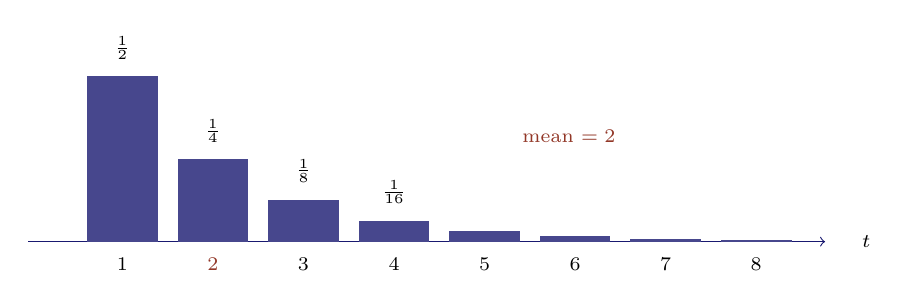
\begin{tikzpicture}[x=1.15cm,y=4.2cm]
  \draw[MidnightBlue,->] (0.35,0) -- (9.15,0);
  \node[font=\scriptsize,anchor=west] at (9.45,0) {$t$};
  \foreach \t/\h in {1/0.5, 2/0.25, 3/0.125, 4/0.0625, 5/0.03125, 6/0.015625, 7/0.0078125, 8/0.00390625} {
    \fill[MidnightBlue!80] (\t,0) rectangle ++(0.78,\h);
  }
  \node[font=\scriptsize,anchor=south] at (1.39,0.52) {$\frac12$};
  \node[font=\scriptsize,anchor=south] at (2.39,0.27) {$\frac14$};
  \node[font=\scriptsize,anchor=south] at (3.39,0.15) {$\frac18$};
  \node[font=\scriptsize,anchor=south] at (4.39,0.085) {$\frac1{16}$};
  \foreach \t in {1,3,4,5,6,7,8} {
    \node[font=\scriptsize,anchor=north] at (\t+0.39,-0.02) {$\t$};
  }
  \node[font=\scriptsize,BrickRed!75!black,anchor=north] at (2.39,-0.02) {$2$};
  \node[font=\scriptsize,BrickRed!75!black,anchor=west] at (5.7,0.32) {mean $=2$};
\end{tikzpicture}
